\documentclass[20pt, a0paper, landscape]{tikzposter}
% \usepackage[utf8]{inputenc}
 
\title{SHARING THE CONSERVATION BURDEN}
\author{Steven Martell$^{\dagger}$, Ian Stewart, Catarina Wor, Bruce Leaman, and James Ianelli $^{\ddagger}$}
\date{\today}
\institute{$^{\dagger}$ International Pacific Halibut Commission, $^{\ddagger}$NOAA National Marine Fisheries Service}
 
\usepackage{blindtext}
\usepackage{comment}

% Themes
\usetheme{Default} 
% \usetheme{Rays} 
% \usetheme{Basic} 
% \usetheme{Simple} 
% \usetheme{Envelope} 
% \usetheme{Wave} 
% \usetheme{Board} 
% \usetheme{Autumn} 
\usetheme{Desert} 


% Block styles
% \useblockstyle{Default}
\useblockstyle{Basic}
% \useblockstyle{Minimal}
% \useblockstyle{Envelope}
% \useblockstyle{Corner}
% \useblockstyle{Slide} 
% \useblockstyle{TornOut}


% Note styles
\usenotestyle{Sticky}


% Note colors
\definecolor{notefgcolor}{named}{black}
\definecolor{notebgcolor}{HTML}{FCF0AD}



% additional packages
% \usepackage{times}
\usepackage{amsmath,amsthm, amssymb, latexsym, bm}
% \usepackage{exscale}
% \usepackage{ragged2e}
% \boldmath
% \usepackage{booktabs, array}
% \usepackage{rotating} %sideways environment
\usepackage[english]{babel}
\usepackage[latin1]{inputenc}
% \listfiles
% \graphicspath{{figures/}}
% \graphicspath{{FIGS/}}




% abbreviations
\usepackage{xspace}
\makeatletter
\DeclareRobustCommand\onedot{\futurelet\@let@token\@onedot}
\def\@onedot{\ifx\@let@token.\else.\null\fi\xspace}
\def\eg{{e.g}\onedot} \def\Eg{{E.g}\onedot}
\def\ie{{i.e}\onedot} \def\Ie{{I.e}\onedot}
\def\cf{{c.f}\onedot} \def\Cf{{C.f}\onedot}
\def\etc{{etc}\onedot}
\def\vs{{vs}\onedot}
\def\wrt{w.r.t\onedot}
\def\dof{d.o.f\onedot}
\def\etal{{et al}\onedot}
\makeatother

\newcommand{\fspr}{F$_{\rm{SPR=35\%}}$}
\newcommand{\bspr}{B$_{\rm{SPR=35\%}}$}
\newcommand{\rspr}{R$_{\rm{SPR=35\%}}$}
\newcommand{\fofl}{F$_{\rm{OFL}}$}

\usepackage{pifont}% http://ctan.org/pkg/pifont
\newcommand{\cmark}{\ding{51}}%
\newcommand{\xmark}{\ding{55}}%

% \newcommand{\fmsy} {F$_{\rm{\textbf{MSY}}}$}
\newcommand{\fmsy}   {$f^*$}

\newcommand{\dye}    { \dfrac{{\partial y_k}}{{\partial f_k}} }%
\newcommand{\dre}    { \dfrac{{\partial R_e}}{{\partial f_k}} }%
\newcommand{\dphi}   { \dfrac{{\partial \phi_k}}{{\partial f_k}} }%
\newcommand{\dphik}  { \dfrac{{\partial \phi_{k'}}}{{\partial f_k}} }%
\newcommand{\dphie}  { \dfrac{{\partial \phi_e}}{{\partial f_k}} }%
\newcommand{\ddphie} { \dfrac{{\partial^2 \phi_e}}{{\partial f_k}^2} }%
\newcommand{\dla}    { \dfrac{{\partial l_a}} {{\partial f_k}}}%
\newcommand{\ddla}   { \dfrac{{\partial^2 l_a}} {{\partial f_k}^2} }%
\newcommand{\ddye}   { \dfrac{{\partial^2 y_k}}{{\partial f_k}^2} }%
\newcommand{\ddre}   { \dfrac{{\partial^2 R_e}}{{\partial f_k}^2} }%
\newcommand{\ddphi}  { \dfrac{{\partial^2 \phi_k}}{{\partial f_k}^2} }%
\newcommand{\ddphik} { \dfrac{{\partial^2 \phi_{k'}}}{{\partial f_k}^2} }%



\definecolor{cM1}{rgb}{0.9608,0.4706,0.4392}
\definecolor{cM2}{rgb}{0.4902,0.6745,0.1216}
\definecolor{cM3}{rgb}{0.2275,0.7765,0.7922}
\definecolor{cM4}{rgb}{0.7765,0.5020,0.9843}


\begin{document}
 
\maketitle

\begin{columns}
	\column{0.250}
	\block{Abstract}{
		The NPFMC recently established new BSAI PSC limits 3,515 mt for Pacific halibut.  This represents a 21\% decrease from the previousl limit of 4,426 mt.  The Council has also requested a discussion paper for its October 2015 meeting exploring ways of indexing BSAI halibut PSC limits to a metric of halibut biomass.  Moving in the direction of jointly managing halibut mortality with variable PSC limits for non-IFQ halibut fisheries will require an allocation agreement between directed and non-directed halibut fisheries.  We propose two options for setting PSC limits: (1) limits based on allocating total catch, and (2) limits based on allocating a proportion of the life-time total mortality rate.  In both options the PSC limits vary in proportion to halibut abundance.  We further demonstrate that option (2) incentivises better resource stewardship where each sector is rewarded with additional catch as efforts are made to reduce the impacts on the Spawning Potential Ratio, or SPR.  We also demonstrate that bycatch mitigation is dynamic and losses to the directed fishery is a function of the relative selectivities, size-at-age, the allocation arrangement, and the harvest policy.  As a consequence, setting PSC limits must jointly address all of these issues.
	}

	% \column{0.25}
	\block{Introduction}
	{
		Annual catch limits for the northeast Pacific halibut fishery are set by the International Pacific Halibut Commission.In Alaska, halibut bycatch mortality is managed under a Prohibited Species Catch (PSC) cap.  Halibut abundance in the Eastern Bering Sea (EBS) is at a record low and the directed fisheries in this region is facing a potential shutdown.  In order to avert the potential crisis, the North Pacific Fisheries Management Council (NPFMC) took final action in June 2015 to reduce the halibut PSC limits by 21\%. 

		Indexing PSC limits to halibut abundance poses several challenges.  First, if the PSC limit is set as a fraction of the available biomass, then a catch sharing plan (allocation) must be specified \emph{a priori}.  The harvest policy for Pacific halibut must reflect this allocation arrangement.  Fisheries reference points (targets, limits, and thresholds), and PSC limits developed in the harvest policy, must also vary with changes in fisheries selectivity, changes in size-at-age, changes in discard mortality rates.

		Mitigation is the process by which the directed fishery catch is reduced to accommodate bycatch fisheries.  Historically, one pound of U26 inch bycatch is approximately equal to one pound of lost yield (O32) in the directed fishery.  This 1:1 ratio was based on an approximation and did not take into consideration the cumulative effects of successive removals and was based on historical size-at-age (coastwide) and historical bycatch selectivities.
	}
	%%
	%%
	% \column{0.25}
	\block{Objective}
	{
		
		\begin{itemize}
			\item Explore ways to index BSAI halibut PSC limits to a metric of halibut biomass.
			\item Describe methods for setting PSC limits based on allocating catch to each sector.
			\item Describe methods for setting PSC limits based on allocating life-time total mortality rate to each sector.
			% \item Use a simple case study with 3 different gear types (selectivities) to 
		\end{itemize}
		 
	}
	%%
% \end{columns}

% \begin{columns}
%     \column{0.4}
%     \block{More text}{Text and more text \blindtext}
 
%     \column{0.6}
%     % \useblockstyle{Slide} 
%     \block{Something else}{Here, \blindtext \vspace{4cm}}
%     \note[
%         targetoffsetx=-9cm, 
%         targetoffsety=-16.5cm, 
%         width=0.35\linewidth
%         ]
%         {e-mail \texttt{stevem@iphc.int}\\
        
%         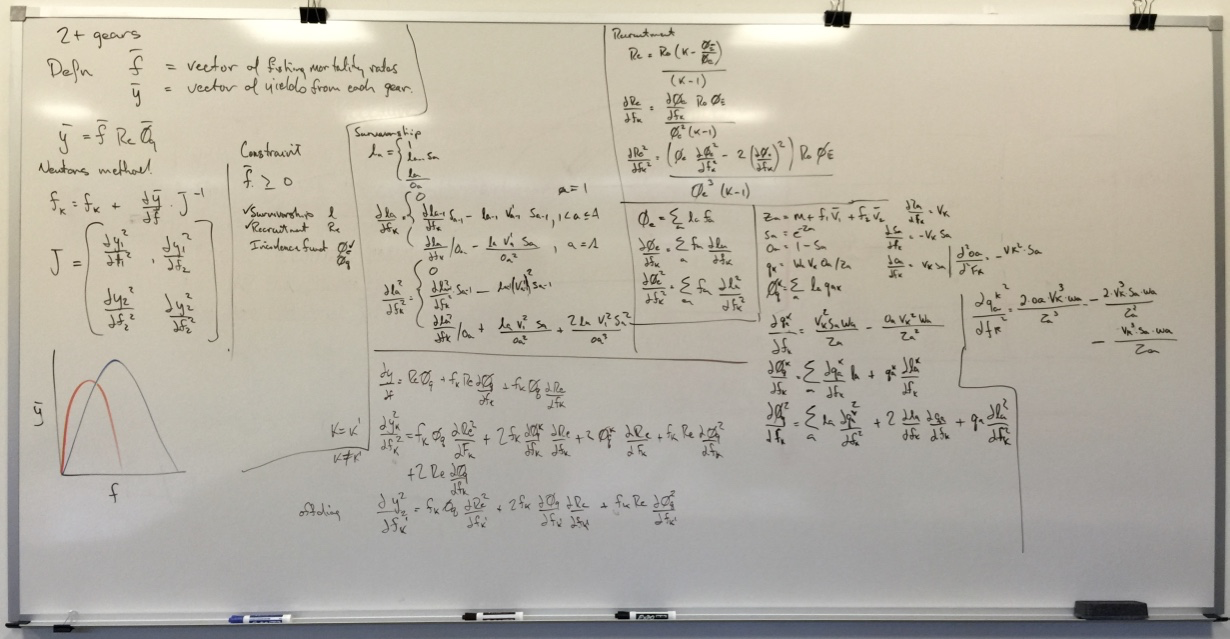
\includegraphics[width=0.95\linewidth,keepaspectratio=true]{./whiteBoard.png}}

% \end{columns}

% \begin{columns}
	\column{0.3}
	\block{Option (1) catch allocation}{
		\begin{itemize}
			\item 
			This option allocates a proportion of the total catch to each sector.  In this case, the total allowable catch (TAC) in each regulatory area is based on the apportioned biomass and the target harvest rate. Each sector (incl.the PSC limit) would receive a portion of the TAC. 
			\item
			Similar arrangements already exist with catch sharing plans, and allocations to the recreational fisheries.
			\item
			Under this option, the IPHC would set the PSC limits on an annual basis once the initial allocation has been established.
		\end{itemize}

	}
	% \column{0.3}
	\block{Option (2)  fishing mortality rate allocation}{
		\begin{itemize}
			\item 

			% This approach also requires an initial allocation agreement, but in this case, what is being allocated is not yield, rather what fraction of the mortality on the spawning potential ratio (SPR) is allocated to each sector.
		\end{itemize}
	}
	\note[]{This is my note}

	\block{Mitigation}{
	Examination of the partial derivatives show how changes in yield from one fishery affect the changes in yield in another fishery.

	\[
	\frac{\partial Y_k}{\partial Y_{\acute{k}}}
	\]
	}

	
	\column{0.250}
	\block{Discussion}{
		There is nothing particular about setting the PSC limits using an abundance based approach versus an SPR-based approach.  It is entirely feasible to determine the proportions for each method that result in the same long term average yield.  What uniquely different between the two approaches is the potential for the SPR-based approach to incentivise behaviour that would maximize the net benefits for all participants in the fishery.  Participants are rewarded for efforts that minimize mortality on the present and future spawning biomass, and by maximizing the yield per recruit,  by recieving a larger portion of the total available surplus.  In contrast, the abundance-based PSC limits has no built in incentive that rewards maximizing the yield per recruit. In fact, if the PSC-limits are in units of weight, then there is an incentive to growth overfish and increase total mortality.  This is also the case for fixed PSC-limits.\\


		In the catch allocation method there is no feedback in the calculations to adjust the PSC limits.  Requires Council intervention to change the PSC limits.  The total mortality rate allocation does have the built in feedback that allows the PSC limits to vary both with abundance and changes in selectivity.
	}
	\useblockstyle{Minimal}


\end{columns}
		
	

\end{document}